\chapter{\textsc{PathObjects} for Squeak Smalltalk}
\label{c:implementation}

\todo[inline]{Introduction}

\section{Data Acquisition}
\todo[inline]{Introduction}

\subsection{Identification of Objects}
\label{ss:ImplementationTracingIdentification}
The fundamental requirement for the reconstruction of object interactions from traces is that object instances can be identified unambiguously.
Unfortunately, the Squeak image does not provide such a functionality out of the box.
Though objects do have an \inlinecode{identityHash} attribute, the value of this attribute is neither unique nor stable \cite{goldberg_smalltalk-80:_1983}.
In the virtual machine we used, it is derived from the least significant bits of the object pointer which is managed by the virtual machine and represents the object's address in main memory.
Hence, the value of the object pointer and thus the value of the \inlinecode{identityHash} are subject to change during garbage collection, which may cause objects to be moved in main memory.
Furthermore, since the \inlinecode{identityHash} uses only the 12 least significant bits, there is no guarantee that two objects that are not referential equal cannot share a common hash value \cite{goldberg_smalltalk-80:_1983}.

The Squeak image does not offer a convenient way to access the object pointers, which could serve as unique identifier for objects.
There are workarounds that would allow to determine its value, but since this value still is subject to change during a tracing run due to the reasons pointed out above, it would require to disable garbage collection during this time span.
This could have undesired side effects, like excessive memory consumption or slow execution speeds due to increased memory allocation effort.

For these reasons, we chose a different approach that allows us to generate unique, stable identifiers for objects.
It exploits the fact that that a comparison for referential quality provided by the \inlinecode{==} method will always yield the correct result.
It returns true if the two objects have the same object pointer, and false otherwise.
Squeak provides a \inlinecode{WeakKeyIdentityDictionary} that has two beneficial properties for our use case.
First, it uses \inlinecode{==} comparison to test dictionary keys for equality.
That means that when using the objects that occur during tracing runs as keys, it is guaranteed that no two objects will be identified as the same key, and an object will always be mapped to the same key once it is present in the dictionary.
The second property is that it uses weak references to manage keys, which implicates that garbage collection of an object is not suspended by the fact that it is used as key in a dictionary.

Consequently, this allows us to use the objects occurring during tracing runs as keys, without interfering with the test execution.
Identifiers can be assigned to objects as values of the dictionary.
Thus, it is guaranteed that one object will always be mapped to the same identifier.
To ensure that no identifier is assigned to two referentially different objects, it is sufficient to use a continuously incrementing integer counter when assigning new identities, or respectively adding new entries to the dictionary.

Since we presuppose that test cases are strictly deterministic (cf. Section \ref{s:DiscussionLimitations}), this strategy results in another benefit.
Namely, objects will always be assigned the same identifier in different tracing runs, since the identifier is only dependent on the relative position in which objects occur for the first time in a trace.
In other words, to stick to the observer example, the instance of \inlinecode{DigitalClock} will always be assigned with the identifier \inlinecode{27} no matter how often the test is executed, since it is the 27th object that occurs in the trace.
This is an important property and prerequisite for the tracing and mapping of outbound object pointers (cf. Section \ref{ss:ImplementationTracingReferences}).

The current implementation constructs a new dictionary of identifiers for each test execution.
But it would also be possible to share identifiers of long living objects like classes across all tracing runs, if a global dictionary were used.
However, we are unaware of a use case that could exploit this possibility, and additional measures would be required to ensure the property described in the previous paragraph.
For that reasons, we favored trace-local over global identity generation.

\subsection{Tracing Approach}
\label{ss:ImplementationTracingApproach}

\begin{figure}
	\centering
	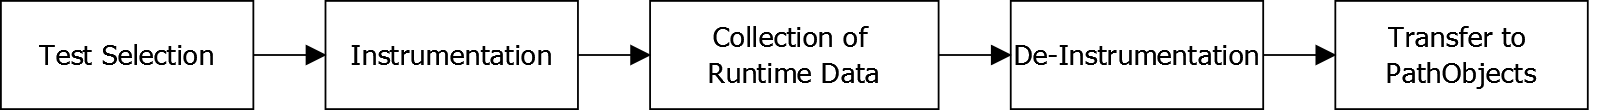
\includegraphics[width=0.9\textwidth]{../images/04-Tracing}
	\caption[TOC Caption]{Tracing foo}
	\label{fig:ImplementationTracing}
\end{figure}

Figure \ref{fig:ImplementationTracing} depicts the fundamental steps that are performed by the \textsc{PathTools} tracing framework to generate an execution trace.
First, the user selects a test case she wishes to analyze.
For instance, this can be done through the test coverage information

Method wrappers offer a convenient way to intercept the execution of specific methods.
As the name suggests, they wrap instances of \inlinecode{CompiledMethod} and take their place in the method dictionary of the corresponding class.
They can be utilized to execute code before and after the invocation of the wrapped method.
Furthermore, they allow the inspection and manipulation of arguments as well as of the return value of a message send.
Thereby, the operation of method wrappers is fully transparent for the callers of wrapped methods.

In order to be suitable for the purposes of \textsc{PathObjects}, the tracing framework had to be extended in two places.
First, a custom \inlinecode{MethodWrapper} had to be implemented that collects the information required for the reconstruction of object interactions.
For each wrapped executed method, this specialized wrapper reports integer identifiers of the receiving object, of the method arguments, and of the return value to the tracer.
Thereby, argument objects are flattened.
That means that if collections of objects are used as arguments, the identifiers of the objects contained in a collection are reported in addition to the identifier of the collection object itself.
Note that an identifier for the sender of a message is not captured, since it would require the expensive operation of stack inspection.
However, this information can be easily reconstructed from the tree structure of the traces, since the sender of a message is identical to the parent element of a call node in the call tree.

The second extension that had to be made is the implementation of a custom \inlinecode{Tracer} that provides some functionality required by our method wrappers and for additional refinement runs.
It provides an implementation of our object identification approach (cf. Section \ref{ss:ImplementationTracingIdentification}) that is used by the method wrappers to generate unique and stable identifiers for objects that occur during tracing.
Furthermore, it provides entry points for the exploration of outbound object references, and is responsible for the execution of refinement runs that are necessary to collect this information (cf. Section \ref{ss:ImplementationTracingReferences}).

\subsection{Reference Tracing}
\label{ss:ImplementationTracingReferences}

\section{Analyses}

\section{Visualization}
\subsection{Graph Layouting}
\subsection{Information Layers}